\documentclass[a4paper,10pt]{article}

%\usepackage{natbib}
\usepackage{amsthm}
\usepackage{amsfonts}
\usepackage{amssymb}
\usepackage{amsmath}
\usepackage{latexsym}
\usepackage{graphicx}
\usepackage{blindtext}

\usepackage{doc}

\newtheorem*{theorem}{Theorem}
\theoremstyle{definition}
\newtheorem*{definition}{Definition}

\hoffset -1in \topmargin 0mm \voffset 0mm \headheight 0mm
\headsep0mm
\oddsidemargin  20mm     %   Left margin on odd-numbered pages.
\evensidemargin 20mm     %   Left margin on even-numbered pages.
\textwidth   170mm       %   Width of text line.
\textheight  252mm

\makeatletter
\renewcommand\@openbib@code{%
     \advance\leftmargin  \z@ %\bibindent
      \itemindent \z@
     % Move bibitems close together
     \parsep -0.8ex
     }
\makeatother

\makeatletter
\renewcommand\section{\@startsection {section}{1}{\z@}%
                                   {-3.5ex \@plus -1ex \@minus -.2ex}%
                                   {1.5ex \@plus.2ex}%
                                   {\large\bfseries}}
\makeatother

\makeatletter
\renewcommand\subsection{\@startsection {subsection}{1}{\z@}%
                                   {-3.5ex \@plus -1ex \@minus -.2ex}%
                                   {1.5ex \@plus.2ex}%
                                   {\normalsize\bfseries}}
\makeatother

\makeatletter
	\setlength{\abovecaptionskip}{3pt}   % 0.25cm 
	\setlength{\belowcaptionskip}{3pt}   % 0.25cm 
\makeatother

\begin{document}
\pagestyle{empty}

\begin{center}
{\bf \Large ROZHRANÍ MOZEK-POČÍTAČ}
\end{center}

\smallskip
\begin{center}
{\large Patrik Lindner}
\end{center}

\smallskip
\begin{center}
Faculty of Mechanical Engineering, Brno University of Technology\\
Institute of Automation and Computer Science\\
Technicka 2896/2, Brno 616 69, Czech Republic\\
Name.Surname@vutbr.cz\\
\end{center}

\bigskip
\noindent Abstrakt: \textit{S rozhraním člověk-počítač se setkáváme denně, a to v nejrůznějších situacích., Jedná se zejména o rozhraní jako je klávesnice, myš či dotyková obrazovka k ovládání elektronických zařízení. Roste však potřeba zajistit možnost užití elektronických zařízení v situacích, kde využití klasického rozhraní není možné. Právě takovouto možnost se snaží poskytnout přímé rozhraní mozek-počítač (brain-computer interface BCI). Toto rozhraní se skládá ze speciálního komunikačního kanálu, který reprezentuje mozkové signály jako informace vnějším zařízením. V současnosti je možné touto metodou ovládat robotické rameno. Ovšem provádění úkonů, jako je přiblížení se k objektu a jeho uchopení, je velmi složité, jelikož současná technologie rozhraní mozek-počítač nesplňuje požadavky na přesnost manipulace s robotickým ramenem. Ke zlepšení přesnosti manipulace pak lze využít spojení tohoto rozhraní se strojovým viděním. Tato technologie se vyvíjí zejména díky jejímu potenciálnímu využití ve zdravotnictví a průmyslu.}

\vspace*{10pt} \noindent Klíčová slova: \textit{Rozhraní mozek-počítač, komunikace, EEG, vizuálně evokovaný potenciál v ustáleném stavu (SSVEP), P300, motorická představivost (MI); neuroprotézy, ovládání robotů.}

\bigskip
\section{Úvod}
\label{sec:1}
Rozhraní mozek-počítač je metoda komunikace mezi uživatelem a zařízením, která je založena na aktivitě neuronů v mozku. Tato komunikace je nezávislá na stavu uživatelových výstupů mozku jako jsou nervy a svaly. Vytváří nový umělý výstup za účelem obnovení či nahrazení přirozené funkce centrální nervové soustavy nebo za účelem ovládání vnějšího zařízení. Nový výstup se realizuje na základě dobrovolného požadavku uživatele a je pod jeho kontrolou. Ve zdravotnictví se tato metoda využívá k pomoci pacientům s úplnou či částečnou ztrátou mobility. Detekcí mozkem generovaných signálů a jejich interpretací umožňuje tato technologie kontrolu kolečkových křesel, umělých končetin a jiných vnějších zařízení, jako jsou exoskelety a ramena robotů za pomoci myšlenek. Kvalita kontroly případné robotické paže však závisí na kvalitě vstupních signálů a počtu stupňů volnosti. Plnění úkolů, jako je přiblížení se k objektu a jeho uchopení, vyžaduje neustálou vzájemnou kontrolu poloh. Avšak aktuální stav rozhraní mozek-počítač ještě není schopen poskytnout dostatečně kvalitní výstupy k tomu, aby bylo dosaženo dostatečně precizního ovládání robotického ramene. Zejména ekonomicky dostupnějšími neinvazivními metodami.

Navzdory jistým obtížím stále dochází k vývoji různých rozhraní mozek-počítač. Podle míry zásahu do lidského organismu lze tato rozhraní rozdělit na invazivní, částečně invazivní a neinvazivní. Invazivní rozhraní se provádí tak, že se elektrody zařízení implantují přímo na mozkovou tkáň. Při částečně invazivním provedení se elektrody implantují na lebku z vnější či vnitřní strany, ale nejsou implantovány přímo v mozkové tkáni. Neinvazivní provedení využívá k detekci signálů z mozku senzorů umístěných na hlavě anebo jiných částech těla. Každé z těchto provedení má jistá pozitiva i negativa.\cite{AI2023obrazovky, article, athanasiou2017rehabilitation, handshake, article3, inbook2, s23136001obrazekmozkusesenzory, s22135000, article4, article2, inbook, zhou2023shared}


\begin{figure}[h]
\begin{center}
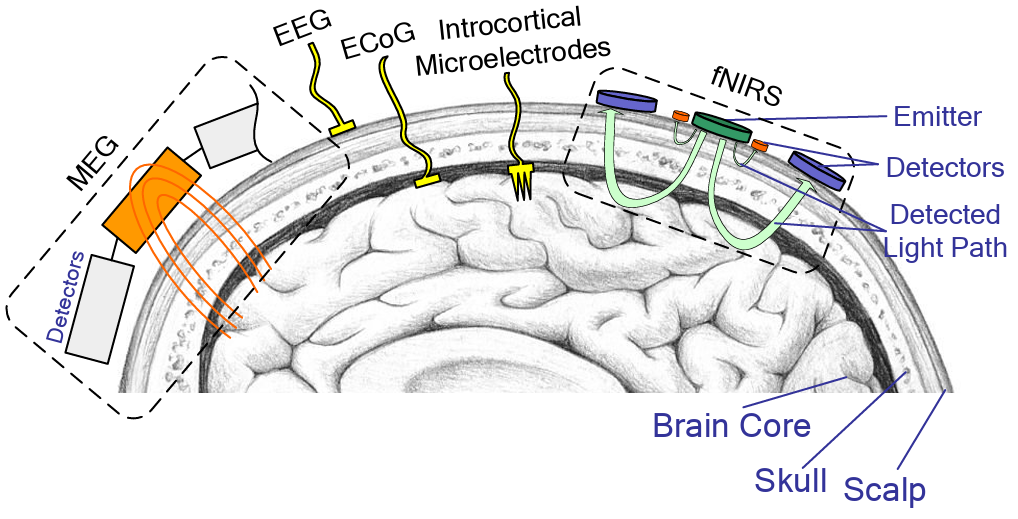
\includegraphics[scale=0.55]{image/umistenisenzorunahlave.PNG}
\caption{Možnosti umístění senzorů: 1) neinvazivní (elektroencefalograf EEG, magnetoencefalograf MEG, near-infrared spektroskopie fNIRS) 2) částečně invazivní (elektrocoticografie ECoG) 3) invazivní (intrakortikální mikroelektrody IM) \cite{s23136001obrazekmozkusesenzory}}
\label{fig:1}
\end{center}
\end{figure}


\section{Techniky měření aktivity mozku}
\label{sec:2}
EEG je neinvazivní technika měření aktivity mozku skrze elektrody umístěné na hlavě s dobrou časovou rozlišovací schopností. Detekuje změny mozkové aktivity v řádu milisekund. Výhody rozhraní na bázi EEG jsou zejména relativně nízká cena a mobilita zařízení. Tato technika má však také své nevýhody. EEG signál je citlivý na šum, je tedy třeba zajistit potřebnou kvalitu signálu. Schopnost systému rozpoznat příkazy uživatele závisí na schopnosti přesně převést EEG data o mozkové aktivitě na informaci, která je pro systém smysluplná. S tím také souvisí nutnost přesné klasifikace signálu, aby byl systém schopný rozpoznat rozdíl, mezi potřebou uživatele pohnout jistou částí těla (palec nahoru vs ukázání ukazováčkem). Oba příkazy by patřily do kategorie pohybu prstem je tedy nutné tuto kategorii ještě více upřesnit a to, tím že každý prst bude také samostatná kategorie. Dalšími výzvami systému EEG je snadno použitelné uživatelské rozhraní, schopnost systému se adaptovat na nejmenší změny v datech EEG a spolehlivost systému vzhledem k dynamickým změnám mozkové aktivity.\cite{AI2023obrazovky, article, athanasiou2017rehabilitation, article3, s23136001obrazekmozkusesenzory}

fNIRS je neinvazivní technika měření aktivity mozku. Využívá část světelného spektra k měření změn v míře okysličení hemoglobinu, která je spojena s aktivitou neuronů. Tato technika je schopna prostorového měření mozkové aktivity, a to i několika oblastí současně, nemá však tak dobrou časovou rozlišovací schopnost jako jiné techniky (EEG). I tato technika má své slabé stránky. Signál fNIRS je slabý a šumem snadno ovlivnitelný. Omezený počet emitorů a detektorů pro prostorové rozlišení způsobuje špatný výklad dat. Vyšší časová rozlišovací schopnost znamená může vést k nevhodnosti využití pro složitější kognitivní úkoly. fNIRS je výrazně dražší nežli EEG či MEG. Systémy fNIRS by při nesprávném použití také mohly poškodit zrak uživatele.

MEG je neinvazivní zobrazovací technika pro záznam aktivity mozku skrze magnetická pole vytvořená elektrickou aktivitou mozku. Časová rozlišovací schopnost je u této techniky dosti vysoká a také poměr signálu k šumu je výborný, což zajišťuje schopnost detekce jemných změn v mozkové aktivitě. Technika MEG je však velmi drahá. Kromě výzkumných pracovišť a nemocnic není její hardware dostupný. Prostorové rozlišení MEG je na nižší úrovni než u ostatních technologií. Tím je snížena přesnost mapování mozkové aktivity. Při pohybu hlavy signály interferují a dochází k nepřesnostem ve výkladu dat, což může být pro uživatele potenciálně nebezpečné.

ECoG je částečně invazivní technika měření aktivity mozku, která má výborné jak časové, tak prostorové rozlišení, díky přímému kontaktu elektrod s neurony. Invazivní lékařský zákrok je však drahý a potenciálně nebezpečný. ECoG má stejně jako ostatní techniky svá úskalí. Signály té to techniky mají poměrně nízkou amplitudu a obsahují jisté množství šumu. Interpretovat data získaná touto metodou může být obtížné vzhledem k tomu, jak komplexní je aktivita neuronů. Tato technika s sebou nese také jistá zdravotní rizika a etické problémy.

Intrakortikální mikroelektrody IM je invazivní technika měření aktivity mozku poskytující vysoké časové a prostorové rozlišení, potřebné pro přesnou kontrolu vnějších zařízení. Tato technika dokáže zaznamenávat aktivitu populací neuronů určitých oblastí mozku či dokonce jednotlivých neuronů samostatně. Do pohybu je zapojeno více mozkových oblastí, což je důležité pro správnou interpretaci informací při přechodu od rozhodnutí v mozku k uskutečnění pohybu vnějšího stroje. Pro precizní pohyb je tedy nutné specifikovat oblasti mozku, jejichž aktivitu je nutné touto technikou sledovat. Největšími výhodami této technologie je její rychlost a preciznost. Ve srovnání s předchozími technikami má tato nejvyšší účinnost. Nevýhodou je extrémně vysoká cena a riziko při implantování zařízení.

Nejpoužívanější z výše uvedených technik je v současné době EEG díky nízké ceně, snadnému nastavení, dobré přesnosti, časové rozlišovací schopnosti s přesností na milisekundy a tomu, že se nejedná o invazivní techniku. Z těchto důvodů se jedná o nejvhodnější metodu zejména pro motoriku a také řeč. Technika by však měla být volena s ohledem na její využití a pohodlí uživatele.\cite{AI2023obrazovky, article, athanasiou2017rehabilitation, article3, s23136001obrazekmozkusesenzory}

\newpage
\section{Paradigmata}
\label{sec:3}

Rozhraní mozek-počítač jsou nejčastěji založeny na paradigmatech P300, vizuálně evokovaný potenciál v ustáleném stavu (steady-state visual evoked potential SSVEP) a motorické představivosti (motoric imagery IM). Existují však i další možná paradigmata.

Paradigma P300 využívá záznamy z EEG aby systém rozpoznal, kdy uživatel reagoval na konkrétní událost či podnět mezi ostatními podněty. Podněty, na něž uživatel reagoval, poté vyhodnotí a odhadne jeho záměr. Výhody tohoto paradigmatu jsou vysoké rozlišovací schopnosti, jednoduché použití. Nevýhodami je dlouhá doba odpovědi systému na podnět kvůli náročnosti zpracování signálů a omezeným počtem kanálů k jeho záznamu a náchylnost na interferenci s okolním šumem.

Vizuálně evokovaný potenciál v ustáleném stavu (SSVEP) využívají blikajícího světla o určité frekvenci a pomocí EEG čtou odezvu mozku na jednotlivé frekvence. Uživatel se zaměří na blikající čtverce na různých místech displeje a mozek na jednotlivá blikání vytvoří jedinečnou reakci. Tímto lze sledovat pohyb očí uživatele bez jakéhokoli dalšího zařízení (kamery). Generované záblesky mají vysokou frekvenci, na kterou si uživatel jednoduše zvykne což předchází vzniku chyb v reprezentaci informace a ovládání robota. Rychlost reakce robota na podnět je také vyšší nežli u P300 díky jednoduchosti zpracování dat signálu. SSVEP je nejužitečnější zejména v průmyslové robotice, automatizovaném dozoru, virtuální a rozšířené realitě a výzkumu umělé inteligence a herních technologií. Hlavními výhodami toho paradigmatu tedy je jeho jednoduchost a rychlá reakce výstupu na vstup. Nevýhodami je nízká míra flexibility, nutnost jistých předem definovaných podmínek a nutnost kalibrace. Dalším problémem je, že uživatel přechází pohledem z příkazového čtverce na objekt manipulovaný robotem, čím dochází ke ztrátě příkazu a nepřesnostem. Možným zkoumaným řešením, které přineslo zlepšení je, že se příkazové čtverce přesunou do okolí manipulovaného objektu a posunují se spolu s ním.


\begin{figure}[h]
\begin{center}
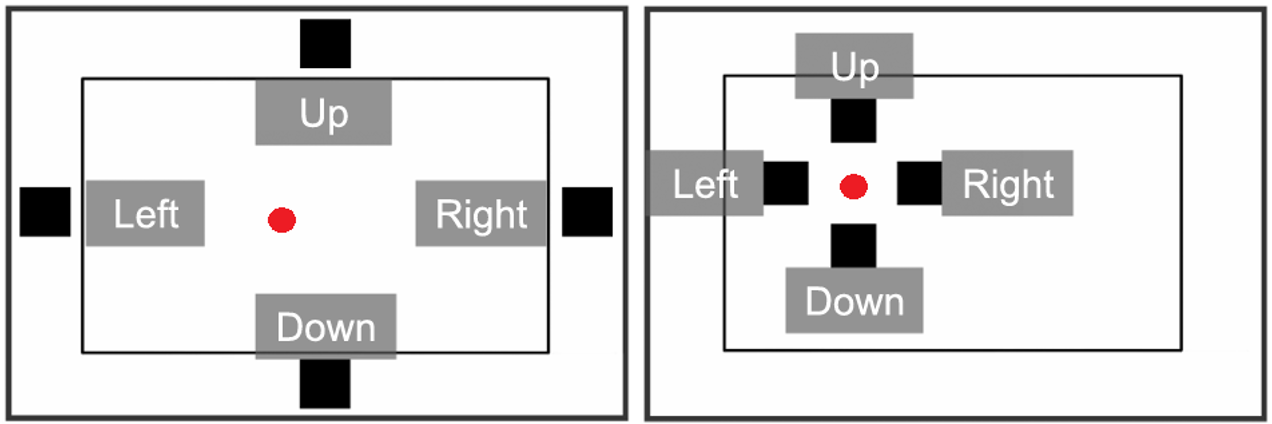
\includegraphics[scale=0.5]{image/trackobektu.PNG}
\caption{klasické SSVEP na obrazovce (vlevo), SSVEP v blízkosti objektu se synchronizovaným pohybem (vpravo) \cite{AI2023obrazovky}}
\label{fig:2}
\end{center}
\end{figure}

Motorická představivost (MI) je paradigma, při kterém si uživatel představuje pohyb jistou částí těla, ale bez skutečného pohybu touto částí těla. Představované pohyby jsou zaznamenány na EEG. Z těchto změn se později zjišťují záměry uživatele k ovládání vnějšího zařízení jako je invalidní vozík, robotická paže, exoskelety či jiná protetika. Největší potenciální míru využití má tedy tato technologie ve zdravotnictví, robotice a zábavním průmyslu. Hlavními výhodami tohoto paradigmatu je široká škála možného využití u lidí s omezenou mobilitou, jednoduché zpracování signálu a relativně nízká cena. Nevýhodami je obtížnost rozlišení skutečného a představovaného pohybu. Navzdory výhodám paradigmatu mohou být komplexnější úkoly těžko proveditelné kvůli vysokému počtu rozhodnutí totiž klesá přesnost jejich intepretace. Dalším problémem je únava uživatele při náročnějších úkolech pak klesá celková efektivita systému.\cite{AI2023obrazovky, s23136001obrazekmozkusesenzory, s22135000, article4, article2, zhou2023shared}

\section{Inovace}
\label{sec:4}
Byl proveden návrh na ovládání robotické paže ovládané na základě SSVEP s pohybujícími se emitory. Cílem bylo snížit potřebu pohybu hlavy a častých změn pohledu mezi objektem určeným k manipulaci a blikajícím podnětem. Ukázalo se, že pohybující se blikající stimuly nemají významný vliv na přesnost dekódování signálu ani amplitudu odezvy. Současná technologie nedokáže zvládnout náročné úkoly v reálném životě. Bylo však prokázáno, že spojením této techniky a mechanismu dvojitého mrknutí (zjišťovaného elektrookulografií EOG) jako spouštěče pro akci uchopení objektu výrazně zlepšuje schopnost uživatele efektivně ovládat připojené robotické rameno. Také uživatelé potvrdili snazší ovládání a nižší mentální zátěž. Tyto výsledky jsou založeny na experimentu sestávajícího se z manipulace více objektů v neuspořádaném prostředí dvanácti uživateli.\cite{AI2023obrazovky}


\begin{figure}[h]
\begin{center}
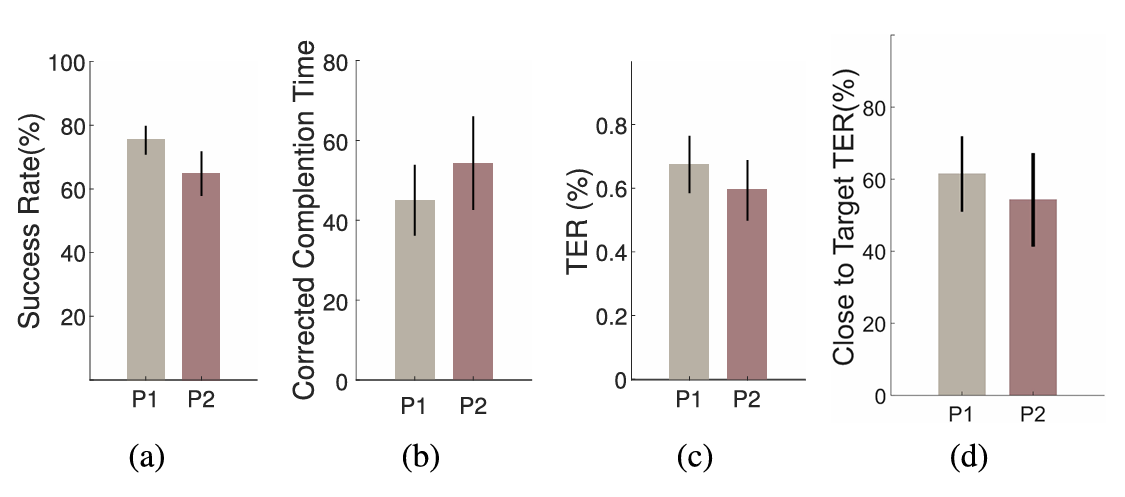
\includegraphics[scale=0.5]{image/srovnanistrackemabez.PNG}
\caption{Srovnání obou SSVEP (P1 nový případ s pohybujícími se stimuly, P2 klasický případ) a) průměrná přesnost plnění úkolu b) průměrný čas dokončení úkolu po korekci (korekce je nutná kvůli odlišným vzdálenostem bodů start cíl) c) poměrná účinnost trajektorie d) poměrná účinnost trajektorie v blízkosti manipulovaného objektu \cite{AI2023obrazovky}}
\label{fig:3}
\end{center}
\end{figure}

\newpage
Pro další zvýšení účinnosti ovládání robotické paže za pomoci rozhraní mozek-počítač, bylo navrženo spojení techniky na základě SSVEP (základní verze) se strojovým viděním. Hybridní model byl zkoušen uživateli v neznámém 3D prostoru a to v asynchronním režimu. Tento režim zajišťuje uživateli kontrolu nad robotickým ramenem a když se objekty objeví v dosahu kamery, strojové vidění pomáhá s prováděním motoricky náročnějších úkonů jako je uchopení objektu a manipulace s ním. Experiment ukázal, že při užití této technologie uživatel přesune rameno na pozici s vysokou přesností. Díky strojovému vidění je pak schopen provést složitou manipulaci, jako je chycení sklenice a pití z ní a to jen s minimálním počtem příkazů a vysokou přesností. Toto řešení také sníží mentální námahu uživatele umožní mu používat systém delší dobu.\cite{zhou2023shared}


\begin{figure}[h]
\begin{center}
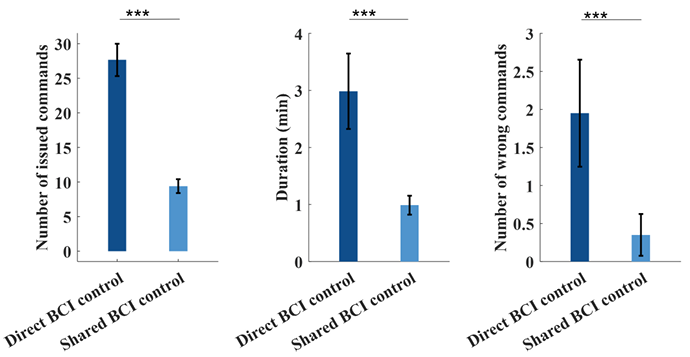
\includegraphics[scale=0.8]{image/strojovevideni.PNG}
\caption{Srovnání výsledků přímé kontroly a hybridní kontroly (hvězdičky značí statistický rozdíl na úrovni tisícin) \cite{zhou2023shared}}
\label{fig:4}
\end{center}
\end{figure}


\section{Aplikace}
\label{sec:5}
V robotice může být rozhraní mozek-počítač použito k ovládání robotických paží, protetických končetin, exoskeletů, humanoidních robotů, či jiných vnějších zařízení. Jako asistenční technologie může pomoci pacientům s omezenou mobilitou a v medicíně se může uplatnit také při diagnostice a rehabilitaci. Rozhraní pomáhá také při komunikaci, přičemž uživatelům s ALS nebo dětskou mozkovou obrnou umožňuje použít ke komunikaci počítač. Další využití má tato technologie v zábavním a herním průmyslu, kde může zlepšit zážitek uživatele. V současné době je však vývoj zaměřen především na robotiku a lékařství.\cite{AI2023obrazovky, article, athanasiou2017rehabilitation, handshake, article3, inbook2, s23136001obrazekmozkusesenzory, s22135000, article4, article2, inbook, zhou2023shared}


\section{Závěr}
\label{sec:6}
Rozhraní mozek-počítač vykazuje v posledních dvaceti letech velký technologický pokrok. Díky přímé komunikaci mozku s vnějším zařízením (robotem) se jedná o zajímavou oblast pro výzkum. Zejména z pohledu zdravotnictví a robotiky (robotické protetické končetiny), jelikož může poskytnout náhradu senzoricko-motorických funkcí. Inovace této technologie poskytují možnost manipulace objektem v neznámém prostředí s vysokou přesností a účinností. Další vývoj této technologie by se měl zaměřit na zpřesnění čtení informací z mozku a jejich interpretaci, zlepšení dostupnosti rozhraní mozek-počítač, zvýšení rozsahu použitelnosti, snížení ceny a zajištění pohodlí uživatele, a to zejména u neinvazivních technik měření mozkové aktivity.

\bigskip
% References
%
\begingroup
\makeatletter
\renewcommand\section{\@startsection {section}{1}{\z@}%
                                   {-3.5ex \@plus -1ex \@minus -.2ex}%
                                   {4.5ex \@plus.2ex}%
                                   {\large\bfseries}}
\makeatother

\nocite{*}
\bibliography{references}{}
\bibliographystyle{plain}
\endgroup



\end{document}